\chapter{Visualizations}
\label{sec:visualizations}
\INITIAL{T}{his section aims} to provide an examination of the methods used to visualize each of the most common types of data in this work. Rather than comprehensively examining all available visualizations, focus will be placed on those data types and structures which are expected to be regularly encountered. These are the data types which are not only most regularly encountered in general, but are particularly applicable to the types of computation scenarios well-suited to analyses in a map-reduce context. 
 
%%%%%%%%%%%%%%%%%%%%%%%%%%%%%%%%%%%%%%%%%%%%%%%%%%%%%%%%%%%%%%%%%%%%%%%%%%%%
%%%%%%%%%%%%%%%%%%%%%%%%%%%%%%%%%%%%%%%%%%%%%%%%%%%%%%%%%%%%%%%%%%%%%%%%%%%%

\section{Numerical Data}
\label{sec:numerical_data}
\INITIAL{N}{umerical data is ubiquitous} when it comes to analysis. Almost all tasks which involve any type of computation will have some sort of summary  or statistics to display as a result. This ubiquity has led to a myriad of visualizations being developed for similar tasks, some of which have more merit than others. The key point to consider when visualizing numerical data is to determine the purpose of the visualization. 

\paragraph{Category Comparison}

\paragraph{Trend Examination} 

\paragraph{Summary Statistics}
There are cases where a visualization more complex than a simple table is unnecessary and perhaps even ill-suited. When 

%%%%%%%%%%%%%%%%%%%%%%%%%%%%%%%%%%%%%%%%%%%%%%%%%%%%%%%%%%%%%%%%%%%%%%%%%%%%
%%%%%%%%%%%%%%%%%%%%%%%%%%%%%%%%%%%%%%%%%%%%%%%%%%%%%%%%%%%%%%%%%%%%%%%%%%%%

\section{Text Data}
\label{sec:text_data}
\INITIAL{O}{often text data is paired} with some form of numerical summary, and in many cases there is no need for a specific type of visualization for this scenario. This could be true for a data set with products and sales numbers for example, where the product names could easily be switched with an integer key and no analysis value would be lost. However, when there is semantic value which can be extracted from the text we can apply more specific techniques. Particularly, this is true if if we can present the text data itself in such a way that a viewer can assess the basic features of the data more quickly by reading the text than by using a numerical approach.

\paragraph{Word Clouds}
The most commonly encountered form of text visualization is a word cloud. Word clouds are a specific form of weighted list which were largely propagated through early blogs and websites as a common feature for exploring tags on posts. There are some examples of these visualizations appearing earlier in printed form \cite{Deleuze1987}, but these are generally not for practical analysis purposes. Word clouds can be used to either summarize the frequency with which items occur, or as a categorization method. In a frequency analysis, words within the cloud have their sizes or colours scaled to reflect their associated frequency. Categorization is applied mainly for navigational purposes, with word sizes scaling to the number of subcategories they encompass. Word clouds are often considered sub-optimal for many use cases because they remove context from the analysis and leave too much extraneous information. They still however prove quite practical for identifying flaws or unexpected features of data sets, if not for analysis. 

%%%%%%%%%%%%%%%%%%
\begin{figure}
	\centering
	\label{fig:wordcloud}
	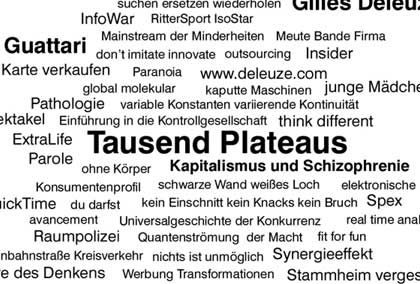
\includegraphics[scale=0.7]{tausend_plateaus_tagcloud.jpg}
	\caption{A word cloud as presented in "Tausend Plateaus: Kapitalismus und Schizophrenie" \cite{Deleuze1987}}
\end{figure}
%%%%%%%%%%%%%%%%%%

\paragraph{Word Trees}
\cite{Wattenburg2008}

\paragraph{Phrase Nets}
Phrase nets \cite{VanHam2009} represent data to some extent in the same fashion as a word cloud, with the size and colour of a word representing it's frequency in the text overall. The added benefit of a phrase net is that it also shows the relationship between words, providing greater context in later stage analyses. Rather than words floating on their own, they are connected by arrows in a directed graph. The arrows are formed based on a predefined relationship between the two and weighted in the same fashion as the words themselves, based on the frequency with which the relationship occurs. Figure \ref{fig:phrasenet} shows a phrase net built using the old testament, which connects two words X and Y based on occurences of the phrase "X of Y" in the text.

%%%%%%%%%%%%%%%%%%
\begin{figure}
	\centering
	\label{fig:phrasenet}
	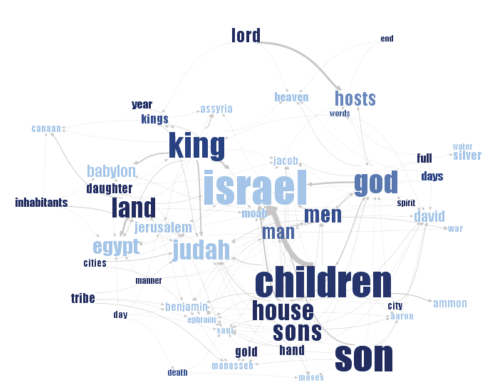
\includegraphics[scale=0.7]{phrase_net.png}
	\caption{A phrase net visualizeing "X of Y" in the old testament \cite{VanHam1987}}
\end{figure}
%%%%%%%%%%%%%%%%%%



%%%%%%%%%%%%%%%%%%%%%%%%%%%%%%%%%%%%%%%%%%%%%%%%%%%%%%%%%%%%%%%%%%%%%%%%%%%%
%%%%%%%%%%%%%%%%%%%%%%%%%%%%%%%%%%%%%%%%%%%%%%%%%%%%%%%%%%%%%%%%%%%%%%%%%%%%

\section{Graph Data}
\label{sec:graph_data}

%%%%%%%%%%%%%%%%%%%%%%%%%%%%%%%%%%%%%%%%%%%%%%%%%%%%%%%%%%%%%%%%%%%%%%%%%%%%
%%%%%%%%%%%%%%%%%%%%%%%%%%%%%%%%%%%%%%%%%%%%%%%%%%%%%%%%%%%%%%%%%%%%%%%%%%%%

